\chapter{Minimal Models}

In the previous chapters, we saw that highest-weight representations of the Virasoro algebra may contain null states for finely-tuned, special values of the central charge \(c\) and the highest weight \(h\). These special values are not accidental mathematical curiosities: they are the fundamental key to the existence of \textbf{rational conformal field theories} (RCFTs), which are theories characterized by a strictly finite number of primary fields.

Among these theories, a distinguished and profoundly important role is played by the \textbf{minimal models}. They provide an infinite, discrete family of exactly solvable two-dimensional conformal field theories (\(\text{CFT}_2\)), and are of central importance both in the study of critical phenomena in statistical mechanics (e.g., the Ising model) and in quantum field theory.

The conceptual architecture underlying minimal models relies on a simple but profound idea:
\begin{itemize}
    \item Generic Virasoro representations contain infinitely many primary fields and an infinite tower of linearly independent descendants.
    \item For special, discrete values of \(c\) and \(h\), singular (null) vectors appear in the Verma modules.
    \item If a sufficient number of null vectors are present, imposing that they strictly vanish (by quotienting out their submodules) truncates the operator algebra. The spectrum of independent primary fields closes under the Operator Product Expansion on a completely \textit{finite} set.
\end{itemize}

This radical truncation is the exact origin of the minimal models. For \(c > 1\), we generally have an infinite number of allowed primary fields, and the theories become tractable only if we assume extended symmetries (such as supersymmetry or W-algebras) beyond the standard conformal symmetry. However, in the region \(0 < c < 1\), the representation theory of the Virasoro algebra alone is so restrictive that it enforces this truncation naturally, completely classifying all possible unitary theories in this domain.

\section{Degenerate Representations}

A highest-weight representation of the Virasoro algebra is technically called \textbf{degenerate} if its Verma module contains at least one null vector.

From our previous analysis of the Kac determinant formula, we know that this degeneracy happens precisely when the highest weight takes one of the roots of the polynomial. Thus, a representation is degenerate when \(h\) assumes one of the special values:
\[
    h = h_{r,s}(c), \quad r, s \in \mathbb{N} \setminus \{0\}.
\]

To systematically chart these roots, a highly convenient parameterization is obtained by introducing an auxiliary parameter \(m\) (which can be real or complex in general, but will be restricted soon for unitarity) such that the central charge is written as:
\[
    c = 1 - \frac{6}{m(m+1)}.
\]
When the central charge is tuned to this form, the specific values of the highest weights that generate null vectors are elegantly expressed as:
\[
    h_{r,s}(m) = \frac{[(m+1)r - ms]^2 - 1}{4m(m+1)}, \quad r, s \in \mathbb{N} \setminus \{0\}.
\]
For any state with these specific weights, the corresponding Verma module contains null vectors and is therefore reducible. The collection of these values \(h_{r,s}\) for a fixed \(c\) is commonly referred to as the \textbf{Kac table}.

\subsection{The Discrete Unitary Series}

We know that for a physical theory to preserve probability, it must be strictly unitary, meaning the Gram matrix must be positive semi-definite at every level, forbidding states with negative norms.

A remarkable foundational theorem in conformal field theory (proven by Friedan, Qiu, and Shenker) imposes devastating constraints on the parameter \(m\). It states that unitary highest-weight representations of the Virasoro algebra with central charge strictly less than one (\(c < 1\)) exist \uline{only for the discrete sequence of integers}:\TODO{put reference}
\[
    c = 1 - \frac{6}{m(m+1)}, \quad m = 3, 4, 5, \dots
\]

For each fixed integer \(m \ge 3\) in this discrete unitary series, the allowed conformal dimensions of the primary fields cannot be arbitrary. They are completely restricted to a finite grid within the Kac table. The integer indices \(r\) and \(s\) defining the allowed weights \(h_{r,s}\) must reside strictly within the bounds:
\[
    1 \leq r \leq m-1, \quad 1 \leq s \leq m.
\]

If we were to plot the curves \(h_{r,s}(c)\) in the \((c, h)\) plane, we would see families of curves intersecting the \(c < 1\) region. The unitary theories sit precisely at the highly specific intersection points where the constraints of positivity simultaneously align, singling out these specific discrete central charges.

These fully classified, exactly solvable unitary theories are mathematically denoted by \(\mathcal{M}_m\) and are called the \textbf{unitary minimal models}. The first member of this series (\(m=3\)) corresponds exactly to the critical Ising model (\(c=1/2\)), the next (\(m=4\)) to the Tricritical Ising model (\(c=7/10\)), and the series continues for models like the 3-state Potts model.

\subsubsection{Number of Primary Fields}

At first glance, the bounds \(1 \le r \le m-1\) and \(1 \le s \le m\) suggest that the Kac table for a given minimal model \(\mathcal{M}_m\) defines a rectangular grid containing \((m-1) \times m\) primary fields.

However, a careful inspection of the formula for \(h_{r,s}\) reveals a crucial internal symmetry. Let us evaluate the conformal dimension for the indices shifted to \((m-r, m+1-s)\):
\[
    \begin{aligned}
        (m+1)(m-r) - m(m+1-s) & = m(m+1) - r(m+1) - m(m+1) + ms \\
                              & = -( (m+1)r - ms ).
    \end{aligned}
\]
Because this term is squared in the numerator of the \(h_{r,s}\) formula, the overall negative sign vanishes completely. Thus, the conformal weights perfectly satisfy the algebraic identification:
\[
    h_{r,s} = h_{m-r, m+1-s}.
\]

This exact degeneracy implies that the labels are subject to the reflection symmetry:
\[
    (r, s) \sim (m - r, m + 1 - s).
\]
Physically, this means that the primary field labeled by \((r,s)\) and the one labeled by \((m-r, m+1-s)\) are fundamentally the exact same representation within the minimal model; they describe the identical state in the Hilbert space.

Because every single field in the grid maps to exactly one other valid field via this reflection, the number of distinct, independent primary fields is exactly half the size of the rectangular grid:
\[
    \text{Number of independent primary fields in } \mathcal{M}_m = \frac{m(m - 1)}{2}.
\]

This result is profoundly important: the number of primary fields is strictly finite, in sharp contrast to generic conformal field theories (where \(c > 1\)). Thus, the adjective ``minimal'' refers precisely to the fact that, for a given allowed central charge, these theories systematically quotient out all null submodules until they contain the absolutely minimal finite set of primary fields compatible with mathematical consistency and unitarity.

\section{The Kac Table}

The allowed primary fields of a unitary minimal model are conveniently arranged in what is universally known as the \textbf{Kac table}. The entries of this table are precisely the allowed conformal weights \(h_{r,s}\) associated with the integer labels:
\[
    1 \leq r \leq m - 1, \quad 1 \leq s \leq m,
\]
modulo the fundamental identification we derived earlier:
\[
    (r,s) \sim (m-r, m+1-s).
\]

To construct the full physical spectrum of a 2D conformal field theory, we should imagine taking this Kac table for the holomorphic sector and ``multiplying'' it by another identical Kac table for the anti-holomorphic sector (\(\bar{h}_{\bar{r},\bar{s}}\)). The complete spectrum is given by the tensor product of these holomorphic and anti-holomorphic representations.

Thus, for each allowed value of the central charge \(c\), we obtain a discrete set of pairs \((h, \bar{h})\) compatible with the unitarity constraints. Once we pair these chiral weights, we can immediately compute the macroscopic physical observables of the primary fields: the \textbf{scaling dimension} \(\Delta = h + \bar{h}\) and the \textbf{conformal spin} \(s = h - \bar{h}\). The Kac table therefore provides an incredibly compact and powerful way to visualize the entire operator content of the theory. Looking at the universality classes generated by these tables, we recognize exact matches with famous statistical mechanics models at criticality (like the Ising model, which is equivalently described by a free Majorana fermion theory when the system is at criticality).

\subsection{Examples of the First Minimal Models}

Let us list and analyze the first few members of the unitary discrete series.

\paragraph{The Trivial Model (\(m=2\)):}
If we formally set \(m=2\), the central charge becomes \(c = 1 - 6/(2 \cdot 3) = 0\). The bounds for the indices are \(1 \le r \le 1\) and \(1 \le s \le 2\), thus the only independent primary field allowed has \(h_{1,1} = 0\) (since \((1,1) \sim (2-1, 3-1) = (1,2)\)). This theory contains only the vacuum state and is physically trivial.

\paragraph{The Ising Model (\(m=3\)):}
From \(m=3\) onwards, we encounter non-trivial unitary theories. The central charges start from \(c=1/2\) and increase monotonically as \(m\) increases, asymptotically approaching \(c=1\) as \(m \to \infty\).
For \(m=3\), the central charge is:
\[
    c = 1 - \frac{6}{3 \cdot 4} = \frac{1}{2}.
\]
We can build the explicit table of values for \(h_{r,s}\) using the formula. The indices run over \(r \in \{1, 2\}\) and \(s \in \{1, 2, 3\}\). The resulting Kac table looks like this:
\begin{table}[H]
    \centering
    \begin{tabular}{c|cc}
        \toprule
        \(3\)   & \(1/2\)  & \(0\)    \\
        \(2\)   & \(1/16\) & \(1/16\) \\
        \(1\)   & \(0\)    & \(1/2\)  \\
        \midrule
        \(s/r\) & \(1\)    & \(2\)    \\
        \bottomrule
    \end{tabular}
\end{table}
As expected, the table is highly redundant due to the symmetry \((r,s) \sim (3-r, 4-s)\). There are only exactly three independent primary fields, with conformal weights:
\[
    h_{1,1} = 0, \quad h_{1,2} = \frac{1}{16}, \quad h_{2,1} = \frac{1}{2}.
\]
These correspond precisely to the three primary fields of the critical Ising model: the identity operator \(\mathbb{I}\) (\(h=0\)), the spin/magnetization operator \(\sigma\) (\(h=1/16\)), and the energy density operator \(\varepsilon\) (\(h=1/2\)). These three primary fields generate the entire spectrum of the theory.

\paragraph{The Tricritical Ising Model (\(m=4\)):}
Setting \(m=4\), we obtain a central charge of:
\[
    c = 1 - \frac{6}{4 \cdot 5} = \frac{7}{10}.
\]
Using the formula for the number of primary fields (\(m(m-1)/2\)), we find that this theory contains exactly six independent primary fields. Physically, this model corresponds to the Ising model with a distribution of \textit{vacancies} (meaning that in some sites on the lattice, the spin is simply absent). Tuning the chemical potential of these vacancies leads to a very rich phase diagram featuring a tricritical point, which falls exactly into this \(c=7/10\) universality class.

\paragraph{The Three-State Potts Model (\(m=5\)):}
For \(m=5\), the central charge is:
\[
    c = 1 - \frac{6}{5 \cdot 6} = \frac{4}{5}.
\]
This unitary minimal series is deeply related to the critical 3-state Potts model. It should be noted that the full physical Potts model is more naturally and compactly described by invoking an \textit{extended} chiral algebra (the \(\mathcal{W}_3\) algebra). Nevertheless, the fundamental minimal-model value of the central charge \(c=4/5\) correctly dictates its foundational structure.

These examples spectacularly demonstrate how abstract representation theory and the purely mathematical minimal models precisely reproduce the macroscopic universality classes of statistical systems at criticality.

\begin{figure}[H]
    \centering
    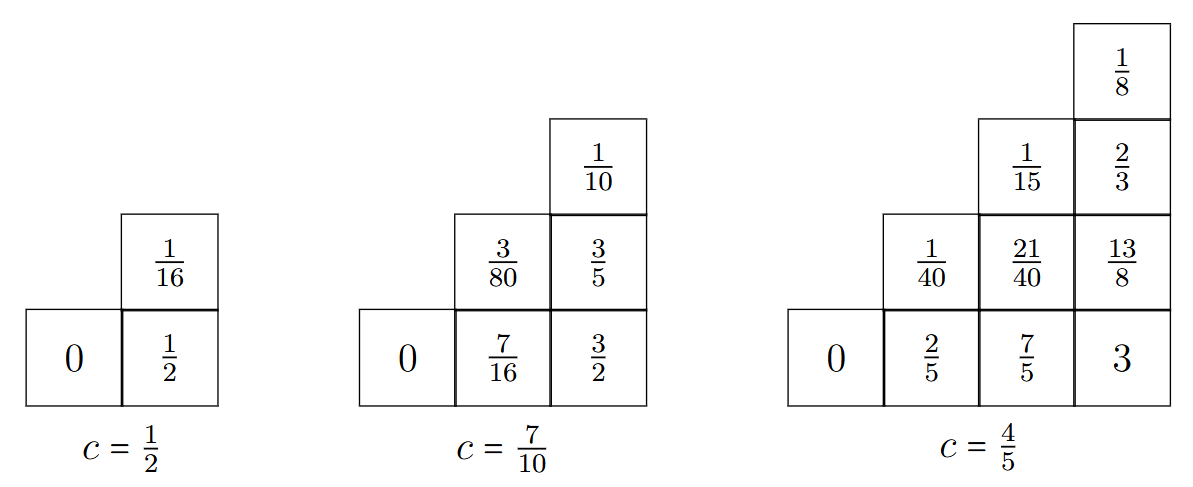
\includegraphics[width=0.8\textwidth]{img/Kac_tables-3mm.png}
    \caption{Kac tables for the first three non-trivial unitary minimal models. Only the entries corresponding to the independent primary fields are reported, while the ones related by the reflection symmetry are omitted. }
\end{figure}

\subsection{Degenerate Fields and Null Vectors}

The absolute defining feature of the primary fields in a minimal model is that their Verma modules are \textit{degenerate}: they are guaranteed to contain null vectors at finite levels in the descendant tower.

Because of the algebraic structure of the Virasoro algebra for these specific discrete weights \(h_{r,s}\), a primary state labeled by the Kac indices \((r, s)\) does not just have one null vector: it typically contains \uline{two independent null states} appearing at specific finite levels. More precisely, the Verma module generated by the field \(\Phi_{(r,s)}\) possesses singular vectors at the exact levels:
\[
    N_1 = rs, \quad \text{and} \quad N_2 = (m - r)(m + 1 - s).
\]

This extraordinarily strong degeneracy is exactly what makes the theory analytically solvable. As we discussed previously, null vectors must strictly decouple from all physical amplitudes. If one inserts a degenerate primary field into an \(N\)-point correlation function, the fact that its descendant at level \(N_1\) (or \(N_2\)) evaluates to zero imposes rigid constraints.

By using the Virasoro Ward identities to replace the descendant modes with differential operators acting on the coordinates of the fields, the decoupling of the null state translates directly into a \textbf{linear differential equation of finite order} (specifically, order \(N_1\) and \(N_2\)) that the conformal blocks must satisfy. Solving these differential equations is one of the main, most powerful computational tools in the study of minimal models, allowing us to find exact analytic results for correlation functions that would otherwise be impossible to compute.

\section{Fusion Rules and Characters of Representations}

A mathematically consistent two-dimensional conformal field theory is strictly not determined merely by listing its allowed set of primary fields and their conformal dimensions. To completely define the local dynamics of the theory, one must also specify exactly how these primary fields interact and combine under the Operator Product Expansion (OPE).

If \(\phi_i\) and \(\phi_j\) are two primary fields in the theory, their generic OPE has the following schematic, highly structured form:
\[
    \phi_i(z, \bar{z}) \phi_j(0, 0) \sim \sum_k C_{ij}^k z^{h_k - h_i - h_j} \bar{z}^{\bar{h}_k - \bar{h}_i - \bar{h}_j} \left[ \phi_k(0, 0) + \sum_{N, \bar{N}} z^N \bar{z}^{\bar{N}} \cdot \text{descendants} \right],
\]
where the leading sum runs over all the primary fields \(\phi_k\) present in the theory. The coefficients \(C_{ij}^k\) are numerical constants defining the coupling strengths, known as the \textbf{structure constants} of the OPE. The exact form of the descendant contributions inside the square brackets is entirely fixed by conformal symmetry acting on the primary fields.

To grasp the global algebraic structure of the theory without writing down the full coordinate dependence and all OPE coefficients, we introduce a powerful, compact notation. We define the \textbf{fusion rules}, which simply count how many times a given conformal family \([\phi_k]\) appears when we ``fuse'' (take the OPE of) the families \([\phi_i]\) and \([\phi_j]\):
\[
    \phi_i \times \phi_j = \sum_k N_{ij}^k \phi_k.
\]
Here, \(N_{ij}^k\) are non-negative integers called the \textbf{fusion coefficients}. If \(N_{ij}^k = 1\), it means the primary \(\phi_k\) (and its descendant tower) appears exactly once in the OPE; if \(N_{ij}^k = 0\), it is strictly forbidden by the symmetries of the theory. The list of allowed primaries on the right-hand side is what we call the fusion rule.

This fusion algebra fundamentally summarizes the representation theory of the Virasoro algebra for the specific model. Minimal models are defined as \textit{rational} conformal field theories precisely because the fusion of any two primary fields always closes on a strictly finite set: the sum over \(k\) is finite.

When computing correlation functions, we use this generalized OPE recursively to reduce \(n\)-point functions to sums over \(3\)-point functions (which depend strictly on the structure constants \(C_{ij}^k\)). Imposing that correlation functions must be single-valued and physically consistent regardless of the order in which we perform the OPEs leads to a highly restrictive set of algebraic equations for the structure constants. This methodology is known as the \textbf{conformal bootstrap}. In minimal models, because the number of fields is finite, the bootstrap yields a closed, exactly solvable set of equations.

\begin{remark}
    A closed, analytic formula for the most general structure constants in minimal models was historically found by Dotsenko and Fateev. Their formula involves complicated contour integrals mathematically expressed via Gamma functions, evaluated exactly in terms of the parameters \(m\), \(r\), and \(s\) labeling the Kac table. This provides a complete, exact mathematical solution to these theories. In non-minimal CFTs, numerical bootstrap methods are instead required to constrain the structure constants.
\end{remark}

\subsection{Fusion Rules in Minimal Models}

Let us consider the most general fusion rule between two arbitrary primary fields \(\phi_{r_1, s_1}\) and \(\phi_{r_2, s_2}\) belonging to the Kac table of a unitary minimal model \(\mathcal{M}_m\) (where the central charge parameter is \(m\)), with the idea to derive the exact set of allowed fields appearing in their OPE.

The exact formula governing their fusion is given by:
\[
    (r_1, s_1) \times (r_2, s_2) = \sum_{\substack{r = |r_1 - r_2| + 1 \\ r \equiv r_1 + r_2 + 1 \pmod 2}}^{\min(r_1 + r_2 - 1,\, 2m - r_1 - r_2 - 1)} \; \sum_{\substack{s = |s_1 - s_2| + 1 \\ s \equiv s_1 + s_2 + 1 \pmod 2}}^{\min(s_1 + s_2 - 1,\, 2m + 1 - s_1 - s_2)} (r, s).
\]

While this expression appears daunting at first glance, its underlying physical logic is incredibly elegant and mirrors familiar concepts:
\begin{itemize}
    \item \textbf{Angular-Momentum-Like Addition:} The lower bound (\(|r_1 - r_2| + 1\)) and the first part of the upper bound (\(r_1 + r_2 - 1\)) strongly resemble the standard Clebsch-Gordan rules for the addition of \(\mathrm{SU}(2)\) angular momenta (or more accurately, quantum spin representations). The labels step by increments of 2, which is enforced by the modulo 2 condition. This condition simply represents parity conservation.
    \item \textbf{Truncation from Above:} If we only had the standard \(\mathrm{SU}(2)\) rules, we could generate arbitrarily large indices by repeatedly fusing fields. However, the upper bounds feature a secondary minimum condition (\(2m - r_1 - r_2 - 1\)). This acts as a strict cutoff. Physically, this \textit{truncation} occurs because the presence of null vectors at specific finite levels systematically annihilates what would otherwise be higher-spin representations.
    \item \textbf{Closure:} Because of this truncation, the result is always a finite sum of allowed primary fields strictly belonging to the original Kac table.
\end{itemize}

For example, if we blindly apply the fusion rules without truncation, we could generate an infinite grid. But the profound constraint imposed by setting the null submodules strictly to zero implies that if we try to fuse fields that would push the index \(r \ge m\) or \(s \ge m+1\), the resulting OPE coefficients are analytically forced to be zero.

Because of this truncation, the fusion rules completely determine the structure of the OPE in minimal models and naturally limit the allowed operator content. Furthermore, because fusing a field with a degenerate field (one containing null vectors) forces the correlator to satisfy a differential equation, we can actually \textit{derive} these fusion rules by analyzing the asymptotic solutions of those very differential equations.

\subsubsection{The Ising Fusion Rules as a First Example}

To see how this works in practice, let us explicitly compute the fusion rules for the critical Ising model (\(m=3\)).

As we established previously, the Kac table for the Ising model features only three distinct primary fields. Using a streamlined notation, we map the Kac labels to their physical operator names:
\[
    \begin{aligned}
        \mathbb{I}  & = (1,1) \quad & \text{with } h = 0 \quad    & \text{(Identity)},           \\
        \sigma      & = (1,2) \quad & \text{with } h = 1/16 \quad & \text{(Spin/Magnetization)}, \\
        \varepsilon & = (2,1) \quad & \text{with } h = 1/2 \quad  & \text{(Energy Density)}.
    \end{aligned}
\]

Using the general fusion formula, let us compute the non-trivial combinations.
First, consider the fusion of the spin operator \(\sigma\) with itself:
\[
    \sigma \times \sigma = (1,2) \times (1,2).
\]
Applying the formula for the \(r\) index (where \(r_1=1, r_2=1\)), the sum runs from \(|1-1|+1 = 1\) to \(\min(1, 6-2-1) = 1\). Thus, \(r=1\) only.
For the \(s\) index (where \(s_1=2, s_2=2\)), the sum runs from \(|2-2|+1 = 1\) to \(\min(2+2-1=3, 7-4=3)\), stepping by 2. Thus, the allowed values are \(s=1\) and \(s=3\).
However, due to the reflection symmetry of the Kac table at \(m=3\), the field \((1,3)\) is identical to \((3-1, 4-3) = (2,1) = \varepsilon\). Therefore, the fusion yields:
\[
    \sigma \times \sigma = \mathbb{I} + \varepsilon.
\]
Physically, this tells us that bringing two spin operators together produces the identity (vacuum) and the energy density operator.

Next, fusing the spin \(\sigma\) with the energy \(\varepsilon\):
\[
    \sigma \times \varepsilon = (1,2) \times (2,1).
\]
The formula forces \(r = |1-2|+1 = 2\) and \(s = |2-1|+1 = 2\). The result is the field \((2,2)\), which by reflection is equivalent to \((3-2, 4-2) = (1,2) = \sigma\). Thus:
\[
    \sigma \times \varepsilon = \sigma.
\]

Finally, fusing the energy \(\varepsilon\) with itself:
\[
    \varepsilon \times \varepsilon = (2,1) \times (2,1).
\]
The formula gives \(r\) from \(|2-2|+1=1\) to \(\min(2+2-1=3, 6-4-1=1)\), forcing \(r=1\). The \(s\) index is forced to \(s=1\). Thus:
\[
    \varepsilon \times \varepsilon = \mathbb{I}.
\]

In summary, the complete set of non-trivial fusion rules for the Ising model is:
\[
    \begin{dcases}
        \sigma \times \sigma           = \mathbb{I} + \varepsilon, \\
        \sigma \times \varepsilon      = \sigma,                   \\
        \varepsilon \times \varepsilon = \mathbb{I}.
    \end{dcases}
\]
These simple algebraic rules already encode a massive amount of information about the physical structure and correlation functions of the Ising critical point. We shall study the profound consequences of these exact rules in detail in the upcoming sections.

\subsection{Characters of Virasoro Representations}

A highly useful and elegant way to compactly encode the entire spectrum of states within a given representation is through its \textbf{character}. For a generic highest-weight irreducible representation \(\mathcal{L}_{c,h}\), the character is defined as the trace of the operator \(q^{L_0 - c/24}\) over the representation space:
\[
    \chi_h(q) = \text{Tr}_{\mathcal{L}_{c,h}} \left( q^{L_0 - \frac{c}{24}} \right).
\]
Here, \(q\) is a formal complex variable (often parameterized as \(q = e^{2\pi i \tau}\) when studying modular invariance on the torus), around which we can expand the character as a power series.

The exponent has a deep physical meaning: \(L_0\) is the dilatation operator (the Hamiltonian in radial quantization), and the uniform shift by \(-\frac{c}{24}\) is related to the Casimir energy of the vacuum state when the conformal field theory is mapped from the complex plane to the cylinder.

If we initially consider a generic \textbf{Verma module} \(\mathcal{V}_{c,h}\) (the representation generated by freely acting with all negative Virasoro modes \(L_{-n}\) on the highest-weight state \(\ket{h}\), assuming strictly \textit{no} null vectors) we can easily compute its character. The result is:
\[
    \chi^\mathrm{Verma}_h(q) = \frac{q^{h - \frac{c}{24}}}{\prod_{n=1}^\infty (1 - q^n)}.
\]
The denominator is precisely the generating function for integer partitions (the Euler function), which perfectly counts the number of ways to distribute the negative modes among the states. The prefactor \(q^{h - \frac{c}{24}}\) accounts for the conformal weight of the ground state and the Casimir energy shift.

If we evaluate the trace explicitly for the true irreducible representation \(\mathcal{L}_{c,h}\), we can group the states by their level \(n\):
\[
    \begin{aligned}
        \chi_h(q) & = \sum_{\ket{s} \in \mathcal{L}_{c,h}} \bra{s} q^{L_0 - \frac{c}{24}} \ket{s} = q^{-\frac{c}{24}} \sum_{\ket{s} \in \mathcal{L}_{c,h}} \bra{s} q^{L_0} \ket{s} \\
                  & = q^{-\frac{c}{24}} \sum_{n=0}^\infty \sum_{\ket{s} \in \mathcal{L}_{c,h}^{(n)}} q^{h+n} \bra{s}\ket{s}                                                        \\
                  & = q^{h - \frac{c}{24}} \sum_{n=0}^\infty \left( \dim \mathcal{L}_{c,h}^{(n)} \right) q^n = q^{h - \frac{c}{24}} \sum_{n=0}^\infty a_n q^n.
    \end{aligned}
\]
The coefficients \(a_n\) precisely count the number of linearly independent physical states at level \(n\) in the irreducible representation. Comparing this expansion with the Verma module character, it becomes evident that the presence of null vectors reduces the number of valid states at each level, leading to a modified counting sequence (\(a_n < p(n)\)).

\subsubsection{Characters in Minimal Models}

In minimal models, the Verma modules are highly degenerate. To obtain the physically relevant irreducible representation \(\mathcal{L}_{c,h}\), we must systematically quotient out all null states. However, because a null state generates its own entire submodule of null descendants, and these submodules can intersect with one another, removing them requires a complex inclusion-exclusion procedure.

This intricate mathematical subtraction is reflected in the explicit character formula for unitary minimal models \(\mathcal{M}_m\), first derived by Rocha-Caridi:
\[
    \chi_{r,s}^{\mathrm{Minimal}}(q) = \frac{q^{-\frac{c}{24}}}{\prod_{n=1}^\infty (1 - q^n)} \sum_{n \in \mathbb{Z}} \left( q^{\frac{[2m(m+1)n + (m+1)r - ms]^2 - 1}{4m(m+1)}} - q^{\frac{[2m(m+1)n + (m+1)r + ms]^2 - 1}{4m(m+1)}} \right).
\]
The infinite sum over \(n \in \mathbb{Z}\) alternating with positive and negative terms (where the second term effectively acts as \(s \to -s\)) exactly accounts for the contributions of the null vectors and their nested intersections.

    [\textit{picture of nested cones representing verma modules and null vectors descendant}]\TODO{add figure of nested cones}

While the foundational classification of the determinant came from Kac, this general character expression was derived by Alvany Rocha-Caridi, one of his students. A deep understanding of the analytical properties of these infinite sums requires the mathematical machinery of \textbf{Theta functions}. The foundational work on such objects by Ramanujan and Hardy has historically been crucial in understanding the modular properties of characters in conformal field theories.

To see the physical effect of this subtraction, consider the state counting at level 2. In a generic Verma module, we have two independent states: \(L_{-2}\ket{h}\) and \(L_{-1}^2\ket{h}\). But in a minimal model, if a null state appears exactly at level 2, the coefficient \(a_2\) in the Taylor expansion of \(\chi_{r,s}^{\mathrm{Minimal}}(q)\) will evaluate to 1 instead of 2. This perfectly reflects the truncation of the Hilbert space.

\subsection{Rationality}

Minimal models are the premier examples of \textbf{rational conformal field theories} (RCFTs). A two-dimensional conformal field theory is called ``rational'' when it satisfies the following incredibly powerful properties:
\begin{itemize}
    \item There is a strictly \textit{finite number} of irreducible representations of the chiral algebra (in this case, the Virasoro algebra).
    \item All local fields in the theory decompose into finite sums of such representations.
    \item The Operator Product Expansion (OPE) explicitly closes on this finite set (the fusion rules generate no new families outside the known set).
\end{itemize}

This is in sharp contrast with generic conformal field theories (\(c > 1\)), which possess infinitely many inequivalent primary fields. The rationality of minimal models makes them both conceptually elegant and completely computationally tractable.

\subsection{Why Minimal Models are Physically Important}

Minimal models are not merely mathematically distinguished curiosities; they provide a direct, exact analytical bridge between abstract representation theory and concrete universality classes in statistical mechanics. Among their most celebrated applications are:
\begin{itemize}
    \item \textbf{The critical Ising model} (\(m=3, c=1/2\)).
    \item \textbf{The tricritical Ising model} (\(m=4, c=7/10\)).
    \item \textbf{Critical points of Potts-like systems} (e.g., the 3-state Potts model at \(c=4/5\)).
    \item \textbf{Certain loop models and restricted solid-on-solid (RSOS) lattice models} at criticality.
\end{itemize}

\subsubsection{Towards the Coulomb Gas Picture}

Finally, we mention that there exists another extremely powerful way to conceptualize and solve minimal models, known as the \textbf{Coulomb gas} or free-field construction. In this framework, one represents the highly interacting minimal-model primary fields in terms of a simple free bosonic field coupled to a ``background charge.''

This alternative approach provides a breathtakingly elegant derivation of both the Kac formula and the fusion rules via contour integrals (the Dotsenko-Fateev integral formalism). While it requires additional mathematical machinery beyond the scope of these notes, it emphasizes a beautiful truth about 2D CFTs: minimal models can be perfectly understood from several complementary points of view, such as purely algebraic (Virasoro algebra and null vectors), analytic (differential equations and conformal blocks), and free-field (Coulomb gas).